\chapter{A Short Guide to the Codebase}
\label{sec:usage}

\section{Directory Overview}

All figures, LaTeX and LibreOffice files for the presentation and this report
are in the respectively named directories. Other important folders are:

\begin{description}
    \item[matlab]
        Contains the full warping pipeline implemented in Matlab. Slow, but useful for debugging and automatic derivation of the Jacobians.
    \item[matlab/input]
        Contains various example scenes for the simulation.
        The courtyard scene was downloaded from \texttt{http://www.luxrender.net/forum/viewtopic.php?f=14\&t=6015} and can be used with LuxRenderer
    \item[cpp] Implementation of all warping code in C++ and a few helpful GUIs to visualize things (including a client for the vi-sensor application).
    \item[arm] Plumbing to run photometric odometry on vi-sensor. All my code is in the 'src/odometry' subdirectory.
\end{description}


\section{Blender Simulation}

For debugging and testing purposes, Blender was used to render images with
disparity data and perfect ground truth.  There are several scenes in
\texttt{matlab/input}. Upon first opening a scene, the ground truth
recording script must be registered once by running the
\texttt{output\_frame\_pos.py} once (or by unsafely reloading the .blend-file by
clicking on the warning in the Blender header menu).

This script will now run every time an animation is rendered and will output
relative camera poses into a CSV file called
\texttt{camera\_trajectory\_relative.csv} in the same directory. Upon first
execution, it will also generate \texttt{camera\_intrinsics.csv} containing all
important parameters of the virtual camera such as focal length and how to
scale the raw disparity values.

The generated CSV files and the rendered images can be read by both the C++ and
the Matlab implementation.


\section{Matlab Implementation}

All Matlab functions generally expect their input data in column matrices (for
example, a list of 100 3D points would have 3 rows and 100 columns). Matlab
only works with simulated data and cannot use raw data from the vi-sensor.

Everything directly implementing warping as described in
section~\ref{sec:warping} can be found in \texttt{core}. This warping pipeline
uses Matlab's matrix operations for speed, but analytically derives the
Jacobians for every iteration, which obviously slows down things immensely.

A good starting point are the scripts in \texttt{test\_scripts}, which provide
various examples of how to use the code: \texttt{run\_minimization.m} runs the
full warping pipeline and Gauss-Newton minimization, while
\texttt{test\_simple\_warping.m} simply plots the warped image for a given
transformation.

Some unit-tests can be run by invocating \texttt{run\_unittests.m} in the root folder.


\section{C++ Implementation}

\begin{figure}[h]
    \centering
    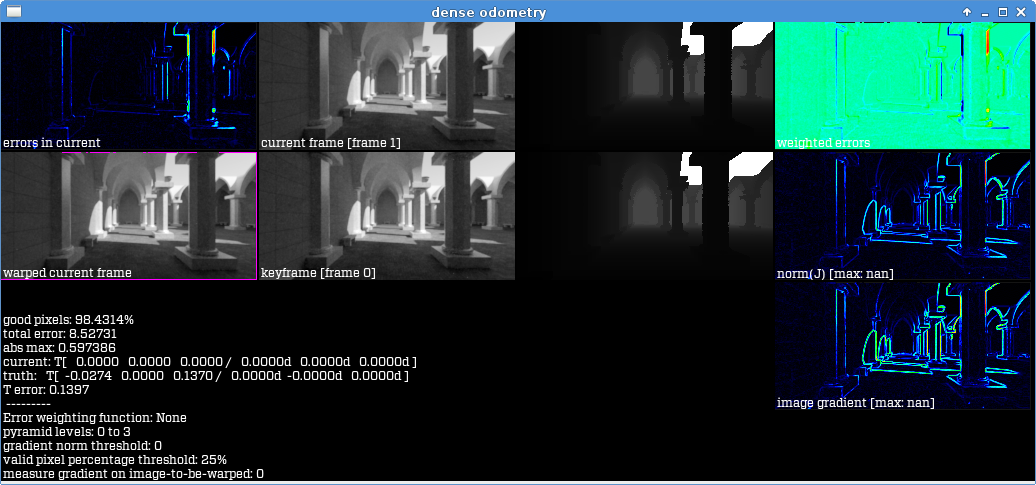
\includegraphics[width=\textwidth]{images/pc_app_screenshot_sim.png}
    \caption{screenshot of simulation view, running with rendered data}
    \label{fig:screenshot}
\end{figure}

The C++ implementation has a lot more features and is siginificantly faster. It
contains various useful tools and visualizations.

To compile and run the application, following libraries are required:

\begin{itemize}
    \item Boost
    \item SFML 2
    \item Eigen 3
\end{itemize}

To compile the code, cmake is used:

\begin{verbatim}
    mkdir build
    cd build
    cmake -D CMAKE_BUILD_TYPE=Release ..
    make dense_odometry
    ./dense_odometry
\end{verbatim}

Specifying \texttt{CMAKE\_BUILD\_TYPE=Release} is optional, but greatly speeds up the code.

Some tests can also be run by calling \texttt{make \&\& make test}.

At the moment, \texttt{main()} has to be manually edited to run the different applications.

There are two implementations of the photometric odometry: A normal one in
\texttt{core/warp.cpp} and \texttt{core/minimization.cpp}, which is modular and
can handle disparity and depth data, and an optimized version in
\texttt{core/warp\_streamlined.cpp} and
\texttt{core/minimization\_streamlined.cpp}, which re-uses as much computation
as possible and only works with disparity data (and therefore cannot be used
with rendered data).

\subsection{simulation}

To view Gauss-Newton minimization in action, trying out different parameters,
rendering cost surfaces etc. call \texttt{run\_minimization()} in main. You can
either load a rendered scene by specifing a scene directory, containing all the
output generated by Blender, or load a rosbag file, containing image and
disparity data.

The simulation view is operated using keyboard shourtcuts:

\begin{description}
    \item[N] advance to next step in scene
    \item[B or Shift-N] go to previous step in scene
    \item[M] enter a rather self-explanatory command-line menu to access other features, such as setting parameter values or rendering a cost-surface plot
    \item[space or P] run or pause minimization
    \item[R] reset current transformation to zero
    \item[T] set current transformation to ground truth
    \item[D] disturb current transformation by a small random amount (can be used to 'unstuck' minimization from local minima)
    \item[F5] run minimization from 0, without live visualization and using the image pyramid
    \item[F6] same as \textbf{F5}, but using the streamlined warping pipeline (only usable for real data with disparity images)
    \item[0] set error weighting function to none
    \item[1-6] set error weighting function to Huber weights, using various parameters
    \item[K] overlay the warped image with the previous image, to visually judge the current transformation
    \item[S] downsample images by a factor of two (moving to the next smaller pyramid level)
    \item[A] reset images to full resolution
    \item[Numpad +/-] scale view, to fit large images on to a small screen or to enlarge downscaled images
    \item[Numpad *] reset view scaling
    \item[Numpad Numbers] translate virtual camera (rotate with CTRL-Numpad)
    \item[F1] save warped image, gradients and Jacobian terms to disk as PNG
    \item[F2] start or stop recording frames into \texttt{recording/} subdirectory
    \item[F12] reset GUI streching after manually resizing window
    \item[ESC] quit
\end{description}



\subsection{live view}

\texttt{show\_live\_data()} shows data from the ARM code running on the vi-sensor. The visensor-node has to be active for receiving live tracking data.

Various keybindings exist:

\begin{description}
    \item[R] clear recorded trajectory and reset orientation
    \item[PageUp/Down] increase/decrease camera shutter time, brightening/darkening the image (this is slow, as a system call has to be made to execute ROS' dynamic\_reconfigure'; Unfortunately no C++ API has been implemented for this)
    \item[Numpad +/-] scale recorded trajectory
    \item[S] manually set shutter time trought terminal
    \item[space] record current frame for later review in simulation view
    \item[return] enter simulation view with recorded frames
    \item[F1] store current trajectory to disk (\texttt{traj\_N.csv})
    \item[F12] reset GUI streching after manually resizing window
    \item[ESC] quit
\end{description}


\subsection{batch processing of recordings}

\texttt{write\_trajectory\_rosbag()} processes a recorded trajectory (either
raw data directly from the vi-sensor, or data processed by OpenCV and
optionally ASLAM). Outputs the tracking data as
\texttt{measured\_trajectory.csv} and optionally ASLAM ground-truth as \texttt{ground\_truth\_trajectory.csv}.

It automatically drops into live view afterwards with frames deemed as 'bad'
(where a big transformation or a lot of iterations were noted, usually
indicating failure of the Gauss-Newton minimization).


\subsection{rendering error surface}

To visualize the photometric error and the Jacobian,
\texttt{draw\_error\_surface()} can be used to render a two-dimensional plot of
cost surface, as for example shown in figure~\ref{fig:costsurface}. This tool
can also be called from live view by pressing \textbf{M} and choosing '12:
render error surface'.

It expects two range parameters for the two plot dimensions. A range parameter
consits of a dimension from 0 to 5, indicating which of the 6 transformation
dimensions to iterate over (x, y, z, alpha/pitch, beta/yaw, gamma/roll), and a
\texttt{linspace()} like range (from, to, number of steps in between).

Depending on the amount of steps, rendering an error plot can take a while.

After the render is done, it is shown on screen and saved to disk. A few commands are available:

\begin{description}
    \item[G] show/hide gradients
    \item[Numpad +/-] scale gradient arrows
    \item[F1 or S] save current view (with gradients, if enabled) to disk
    \item[ESC or Q] quit (and return to live view, if called from there)
\end{description}


\section{ARM code}

The C++ implementation can be cross-compiled to the vi-sensor's ARM Cortex A9
without any modifications by using the Xilinx SDK. The only ARM specific code
is \texttt{src/odometry/odometry.cpp} which initialized the photometric odometry, passes
along the data from camera and FPGA and transmits the tracked movement over the
network.

\subsection{communication between vi-sensor and PC application}

To report the tracked movement, a fake camera is inserted
(\texttt{src/odometry/utils/FakeCamSensor.cpp}) which is received by the
visensor-node which passes it trough the ROS message system as a normal camera
image. The PC app receives everything trough the ROS interface.


\subsection{running the vi-sensor application}

All parameters for the ARM code are set in \texttt{src/odometry/odometry.cpp},
a few important parameters can be overriden via command line tough: Smallest
and biggest pyramid level can be set by using \texttt{--max-pyramid-level N}
and \texttt{--min-pyramid-level N} (a minimum of 2 and a maximum 3 usually
provide good and fast tracking). Transmitting the two camera images and
disparity values over the network can be disabled with \texttt{--no-images},
which speeds up tracking by a few FPS at the cost of not being able to see what
the sensor can see.

It is also important to disable all camera automatics. This can be done trough
the ROS interface by running:

\begin{verbatim}
rosrun dynamic_reconfigure dynparam set /visensor_node "{
        'individual_cam_config': 0, \
        'cam_agc_enable': 0, \
        'cam_aec_enable': 0,  \
        'cam_coarse_shutter_width': 300, \
        'penalty_1': 20, \
        'penalty_2': 200, \
        'threshold': 100, \
        'lr_check': 2 \
    }"
\end{verbatim}

This is also executed by the live viewer application on startup (which can also
be used to manually change the shutter time).


\subsection{timing}

To measure performance, the code has been instrumented to count CPU cycles. To
compile without, make sure \texttt{NO\_TIMERS} is defined. Otherwise,
measurement results are displayd upon stopping the visensor-node on the host
PC.
